\section{Exercise 4 - Binary Tree Algorithms for \texttt{MPI\_Bcast} and \texttt{MPI\_Reduce}}
Instead of “lined up” processes we now want to use a binary tree structure and according algorithms 
\texttt{MY\_Reduce\_T()} and \texttt{MY\_Bcast\_T()} for reduction and broadcasting. As we understand 
each process as a node, we will use the wording node from now on. For indexing of the nodes, we use preorder traversal.

We start very similar to the implementations of \texttt{MY\_Reduce\_P()} and \texttt{MY\_Bcast\_P()} 
from exercise 2. For the reduction \texttt{MY\_Reduce\_P()}  the root node (rank $=0$) on level 0 should 
gain the reduced result. Hence, the leaves start by sending the data block by block to their parents. All 
interior nodes receive exactly two data blocks per communication round. One from their left and one from their 
right child. After performing a local reduction, the data is sent to the nodes parent. In the end, the root 
node receives the data from its two children and ends up with the reduction result. For the broadcast 
\texttt{MY\_Bcast\_P()}, the root node sends the data block wise to its two children. A child receives 
the data and immediately forwards this data to its children, in case it is not a leaf.\\

The trivial combination of \texttt{MY\_Reduce\_T()} and \texttt{MY\_Bcast\_T()} can be seen 
as a pipelined variant of \texttt{MPI\_Allreduce()}.\\

\begin{figure}[h]
    \begin{center}
        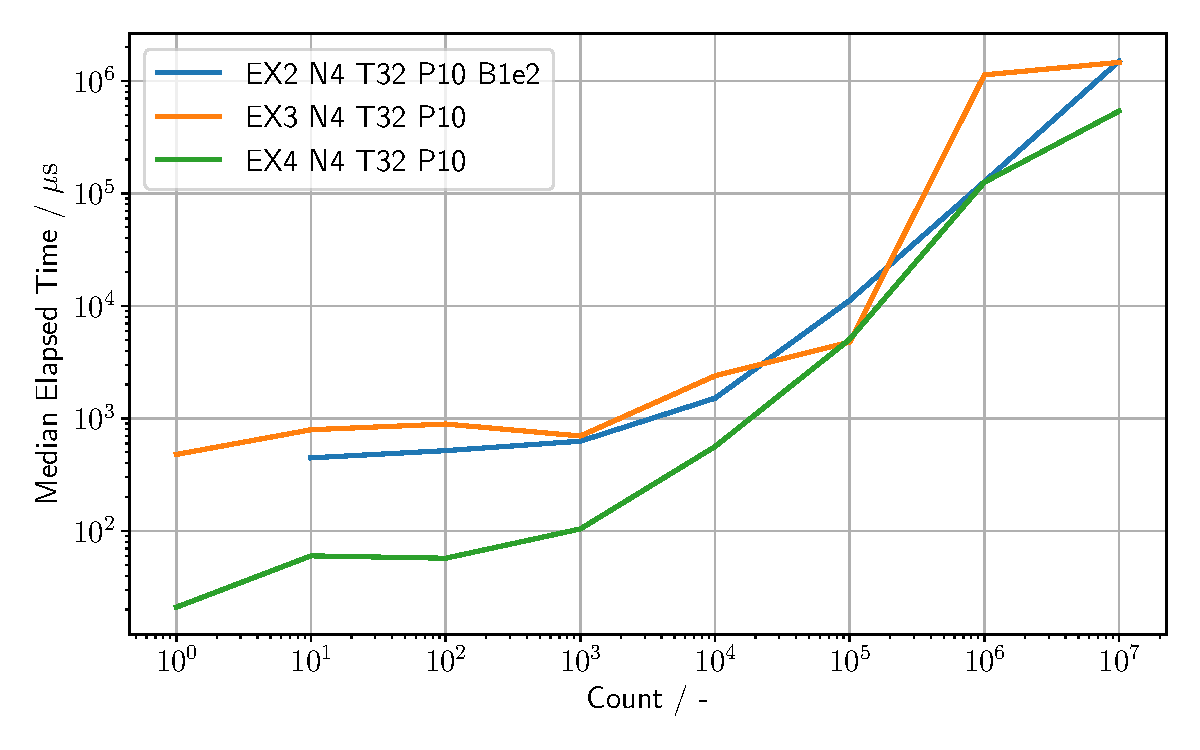
\includegraphics[width=1.0\linewidth]{figures/Ex4_1.pdf}
        \caption{Caption for Ex4 plot 1}
        \label{Ex4_1_p}
    \end{center}
\end{figure}

\begin{figure}[h]
    \begin{center}
        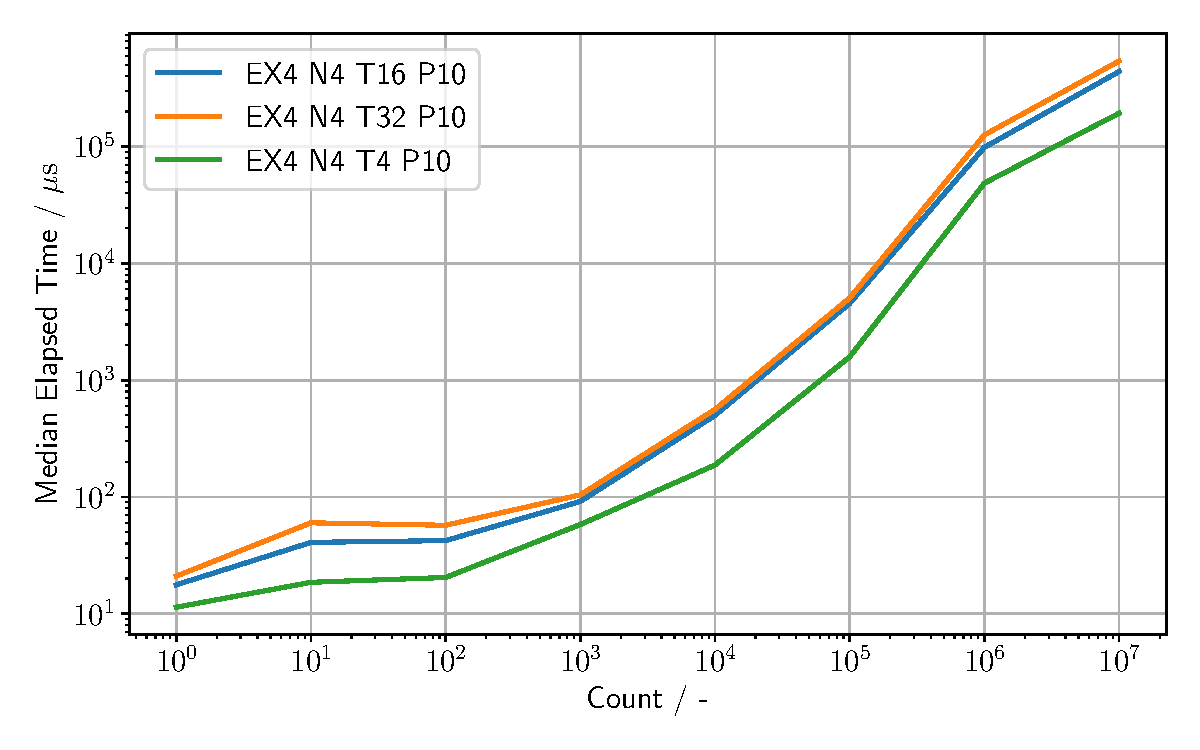
\includegraphics[width=1.0\linewidth]{figures/Ex4_2.pdf}
        \caption{Caption for Ex4 plot 2}
        \label{Ex4_2_p}
    \end{center}
\end{figure}

\begin{figure}[h]
\centering
    \begin{minipage}{.5\textwidth}
        \centering
        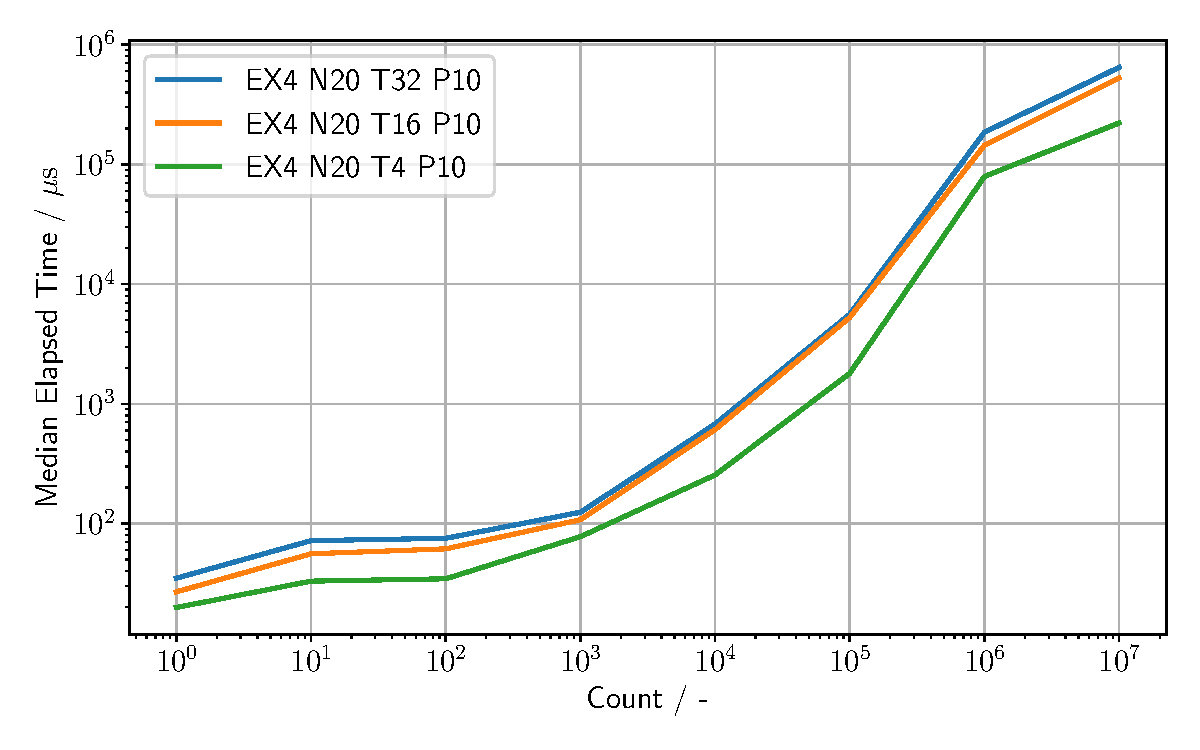
\includegraphics[width=1.0\linewidth]{figures/Ex4_3.pdf}
        \captionof{figure}{Caption for Ex2 plot 3}
        \label{Ex4_3_p}
    \end{minipage}%
    \begin{minipage}{.5\textwidth}
        \centering
        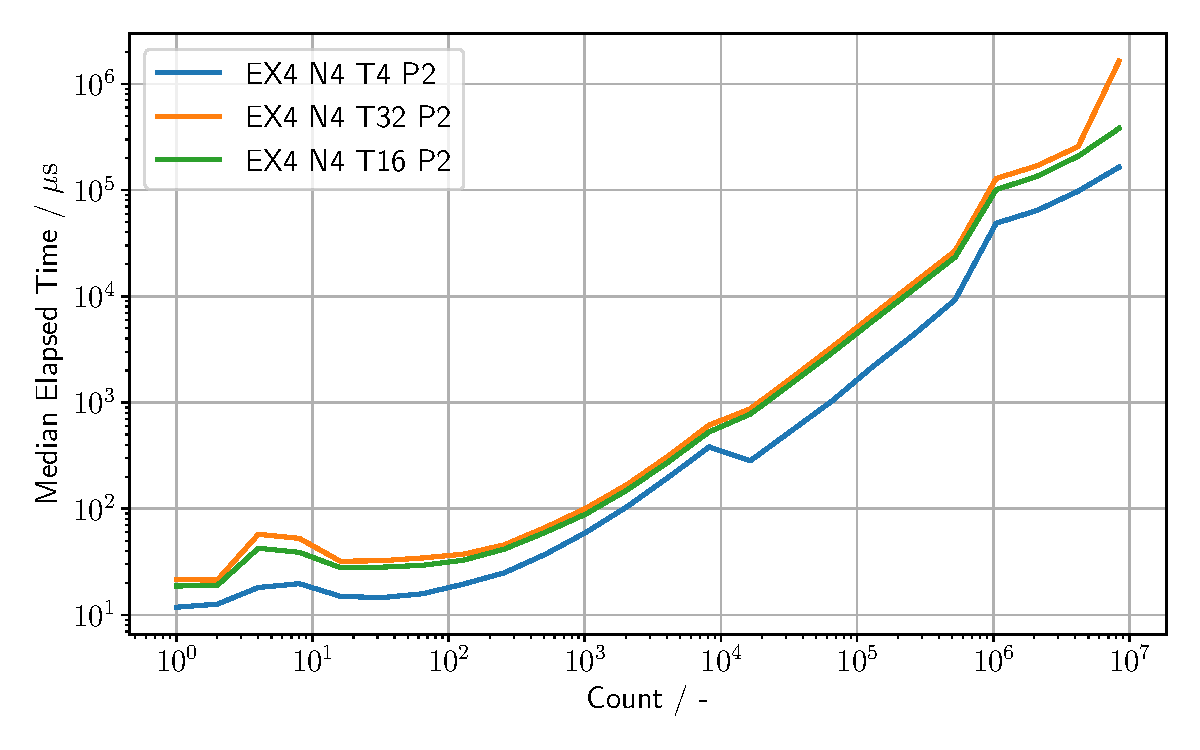
\includegraphics[width=1.0\linewidth]{figures/Ex4_4.pdf}
        \captionof{figure}{Caption for Ex4 plot 4}
        \label{Ex4_4_p}
    \end{minipage}
\end{figure}